\documentclass[11pt]{amsart}

\usepackage[T1]{fontenc}
\usepackage{lmodern}
\usepackage{microtype}
\usepackage{amsmath,amssymb}
\usepackage{booktabs}
\usepackage{graphicx}
\usepackage{xcolor}
\definecolor{linkblue}{RGB}{0,40,120}
\usepackage[colorlinks=true,linkcolor=linkblue,citecolor=linkblue,urlcolor=linkblue]{hyperref}

\graphicspath{{figures/}}

\newcommand{\TVD}{\mathrm{TVD}}

\title[Vetting Collatz anomalies]{Vetting statistical anomalies in the Collatz map:\\ a falsification protocol and four worked failures}

\author{Daniyal Kadirbekov}
\email{daniyal.kadirbekov@gmail.com}

\date{17 June 2026}

\subjclass[2020]{Primary 11B83; Secondary 62A01}
\keywords{Collatz conjecture, $3x+1$ problem, Benford's law, 2-adic valuation, null model, effect size, finite-range artifact}

\begin{document}

\begin{abstract}
Computational studies of the Collatz map regularly report statistical regularities in trajectory data that look like structure in the map and turn out to be artifacts of method. We isolate three failure modes that produce most of them, comparing against the wrong null model, reading a sample-size-inflated significance statistic as an effect, and using an estimator that a few extreme terms dominate, and we propose a three-rule protocol for telling a candidate anomaly from an artifact: fix the null before measuring, report effect sizes rather than significance at large pooled sample sizes, and require any effect to persist rather than decay as the range grows. We apply the protocol to four candidate anomalies in trajectories of starting values up to $10^6$, a Benford ``violation,'' a $2$-adic valuation excess, a prime versus composite stopping-time gap, and a Sophie Germain ratio near $4/3$, and each dissolves. As the hardest case we apply it to our own last surviving conjecture. We had proposed that the small finite-range departure of trajectory leading digits from Benford's law is caused by the low-altitude values every trajectory shares; the protocol's own excision test refutes that mechanism, and what remains is a real but map-specific per-digit residual that decreases monotonically over four decades of range. The contribution is the protocol and the discipline of applying it without exception, including to the conclusion one would prefer to keep.
\end{abstract}

\maketitle

\section{Introduction}

The Collatz conjecture, attributed to Lothar Collatz (1937), concerns the map
\begin{equation}
T(n) =
\begin{cases}
n/2 & \text{if } n \equiv 0 \pmod 2,\\
3n+1 & \text{if } n \equiv 1 \pmod 2,
\end{cases}
\end{equation}
and asserts that iteration of $T$ from any positive integer eventually reaches $1$. The problem is open; Lagarias \cite{lagarias1985} surveys its history, Tao \cite{tao2019} proved that almost all orbits attain almost bounded values in the sense of logarithmic density, and Barina \cite{barina2021} verified convergence for all $n \le 2^{68}$.

Because the conjecture is elementary to state and easy to compute, it attracts a large informal literature that looks for statistical structure in trajectory data: regularities in leading digits, in stopping times, in the behaviour of special classes of starting values. Such regularities are reported in blog posts, in preprints, and in archived work, often as evidence of hidden order in the map. Many do not survive scrutiny, and the reason is rarely arithmetic. It is statistical.

This paper is about how to tell the difference. We isolate three failure modes that, in our experience, generate most of the spurious regularities reported in computational Collatz work.
\begin{enumerate}
\item \emph{The wrong null.} A statistic measured over the integers a process happens to visit is compared against the distribution for integers chosen uniformly, so a feature of the sample is read as a feature of the map.
\item \emph{Significance read as effect.} With pooled sample sizes of order $10^8$, a $\chi^2$ test rejects any fixed null for arbitrarily small deviations, because $\chi^2$ grows linearly in the sample size at fixed effect. A large test statistic is then reported as a large effect. This trap is well documented in the Benford literature specifically \cite{cerqueti2023, kossovsky2021}.
\item \emph{A dominated estimator.} A mean of ratios, or any estimator a handful of extreme terms can dominate, is reported as if it were a stable central tendency.
\end{enumerate}
None of these is novel as a statistical observation. The contribution here is to state them as a protocol, to apply that protocol to four candidate anomalies that we ourselves initially believed, and to show that each dissolves. Claims of these shapes circulate widely in informal treatments of the map. We do not adjudicate any specific claim; we note only the setting in which our four cases, and the protocol that resolves them, belong.

Section~\ref{sec:protocol} states the protocol. Section~\ref{sec:cases} works the four cases. Section~\ref{sec:capstone} applies the protocol to our own surviving conjecture and reports that it fails too. Section~\ref{sec:discussion} draws the general lesson.

\section{The protocol}\label{sec:protocol}

\subsection{Data}
We computed the full trajectory of every starting value $n$ from $1$ to $10^6$, recording the total stopping time $\sigma_\infty(n)$ (steps to reach $1$), the stopping time $\sigma(n)$ (steps to first fall below $n$), and the maximum altitude. Pooling all intermediate values across all trajectories yields $132{,}434{,}424$ values, computed exactly with a memoized recurrence: the statistics of the trajectory of $n$ equal the statistics accumulated until the trajectory first falls below $n$, plus the cached statistics of that smaller value. Every table below is reproducible from a single verification script (Section~\ref{sec:code}).

\subsection{Three rules}
\begin{enumerate}
\item \emph{Correct nulls.} Where a claim concerns the map, the null is the statistic over uniformly random inputs, not over the biased subset of integers that trajectories happen to visit.
\item \emph{Effect sizes, not significance.} We report the total variation distance ($\TVD$) where a distributional comparison is needed, and treat $\chi^2$ as a reference quantity only, since at these sample sizes it measures the sample size.
\item \emph{Persistence under scale.} A genuine structural property should persist or sharpen as the range $N$ grows. An effect that decays monotonically with $N$ is finite-range. We test every candidate at $N = 10^3, 10^4, 10^5, 10^6$, a thousandfold span, so that ``decreases with range'' is a four-point statement rather than a single step.
\end{enumerate}

\section{Four worked cases}\label{sec:cases}

\subsection{Global statistics}\label{sec:global}
Table~\ref{tab:global} collects the records and group means for context; Figure~\ref{fig:scatter} shows the total stopping time scatter.

\begin{table}[ht]
\centering
\caption{Global statistics for starting values $1 \le n \le 10^6$.}
\label{tab:global}
\begin{tabular}{lr}
\toprule
Metric & Value \\
\midrule
Maximum total stopping time & $524$ steps ($n = 837{,}799$) \\
Maximum stopping time & $287$ steps ($n = 626{,}331$) \\
Maximum altitude & $56{,}991{,}483{,}520$ ($n = 704{,}511$) \\
Number of delay records & $43$ \\
Mean $\sigma_\infty$, primes & $136.41$ \\
Mean $\sigma_\infty$, composites & $131.01$ \\
Mean $\sigma_\infty$, odd composites & $137.82$ \\
Mean $\sigma_\infty$, even composites & $125.27$ \\
\bottomrule
\end{tabular}
\end{table}

\begin{figure}[ht]
\centering
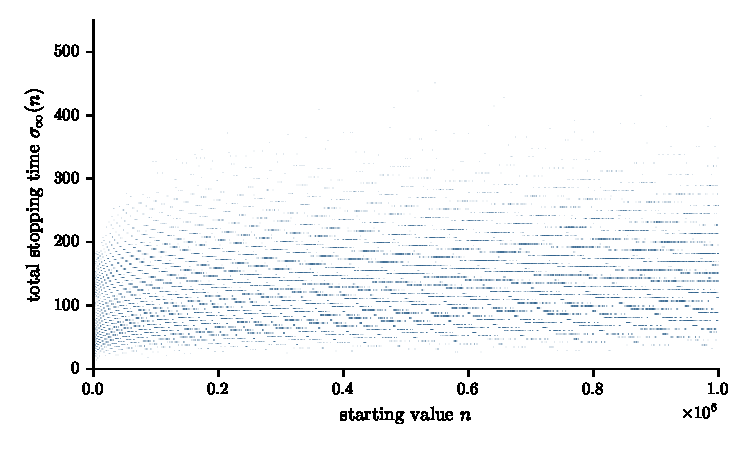
\includegraphics[width=\textwidth]{fig_stopping_times.pdf}
\caption{Total stopping time $\sigma_\infty(n)$ for $n \le 10^6$ (every twentieth value plotted).}
\label{fig:scatter}
\end{figure}

\subsection{Case 1. The Benford ``violation'' is a significance artifact}\label{sec:benford}

Benford's law assigns leading digit $d$ the frequency $\log_{10}(1 + 1/d)$, and Kontorovich and Miller \cite{km2005} proved that suitably formulated Collatz statistics satisfy it asymptotically, with Lagarias and Soundararajan \cite{ls2006} later giving a quantitative finite-length version for single orbits. An earlier version of this analysis declared the opposite, that trajectory leading digits \emph{violate} Benford's law, on the strength of a $\chi^2$ test against a fixed critical value. The trap is general rather than specific to this map \cite{cerqueti2023, kossovsky2021}, and Table~\ref{tab:tvd} shows why the reasoning is empty here. As the range grows, $\chi^2$ rises by a factor of $450$ while the actual deviation, the total variation distance from Benford, \emph{shrinks}. The $\chi^2$ statistic is a measure of the pooled count, not of the effect.

\begin{table}[ht]
\centering
\caption{Scale dependence of the leading-digit deviation. The $\chi^2$ statistic is reported for reference only; at these sample sizes it measures $N$, not the effect.}
\label{tab:tvd}
\begin{tabular}{rrrr}
\toprule
$N$ & Pooled values & $\chi^2$ & $\TVD$ from Benford \\
\midrule
$10^3$ & $60{,}542$ & $1{,}121$ & $0.0444$ \\
$10^4$ & $859{,}666$ & $8{,}140$ & $0.0315$ \\
$10^5$ & $10{,}853{,}840$ & $61{,}154$ & $0.0241$ \\
$10^6$ & $132{,}434{,}424$ & $506{,}395$ & $0.0198$ \\
\bottomrule
\end{tabular}
\end{table}

\begin{figure}[ht]
\centering
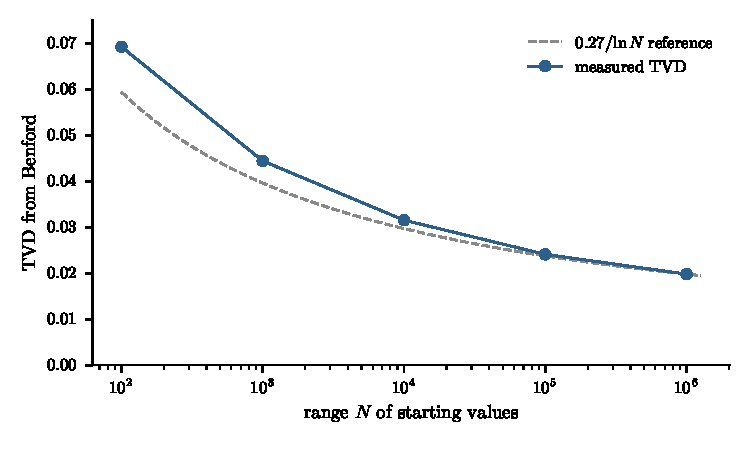
\includegraphics[width=\textwidth]{fig_tvd_trend.pdf}
\caption{Total variation distance from Benford as a function of range $N$. The deviation decreases monotonically, toward the proven asymptotic result rather than away from it.}
\label{fig:tvd}
\end{figure}

The honest statement is that the leading-digit distribution converges \emph{toward} Benford as the range grows. The full per-digit picture at $N = 10^6$ is in Table~\ref{tab:digits} and Figure~\ref{fig:digits}. We do not single out digit $3$: although $3$ is the multiplier of the map, digit $4$ ($+15.0\%$) and digit $6$ ($-12.3\%$) both deviate more than digit $3$ ($-5.0\%$) and admit no such reading, so a digit-$3$ narrative would be post hoc. The size and origin of the residual deviation are the subject of Section~\ref{sec:capstone}, where we test our own explanation of it.

\begin{table}[ht]
\centering
\caption{Leading-digit distribution of all $132{,}434{,}424$ pooled trajectory values, $N = 10^6$.}
\label{tab:digits}
\begin{tabular}{crrr}
\toprule
Digit & Observed & Benford & Deviation \\
\midrule
1 & $0.2985$ & $0.3010$ & $-0.9\%$ \\
2 & $0.1739$ & $0.1761$ & $-1.2\%$ \\
3 & $0.1187$ & $0.1249$ & $-5.0\%$ \\
4 & $0.1115$ & $0.0969$ & $+15.0\%$ \\
5 & $0.0794$ & $0.0792$ & $+0.3\%$ \\
6 & $0.0587$ & $0.0669$ & $-12.3\%$ \\
7 & $0.0574$ & $0.0580$ & $-1.1\%$ \\
8 & $0.0542$ & $0.0512$ & $+6.0\%$ \\
9 & $0.0477$ & $0.0458$ & $+4.2\%$ \\
\bottomrule
\end{tabular}
\end{table}

\begin{figure}[ht]
\centering
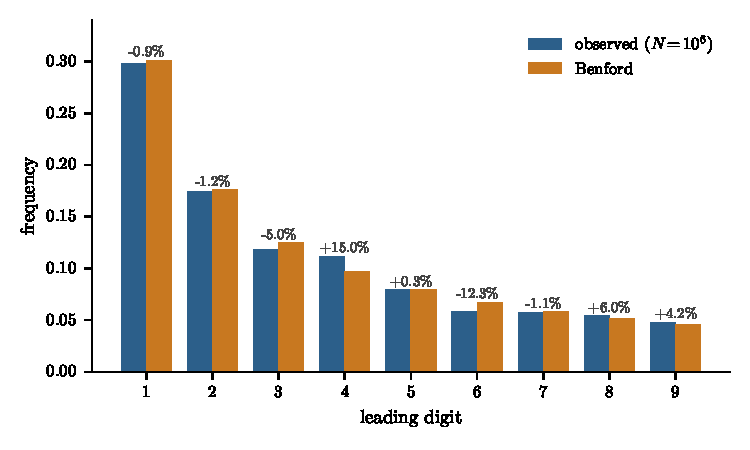
\includegraphics[width=\textwidth]{fig_benford_digits.pdf}
\caption{Observed leading-digit frequencies at $N = 10^6$ against Benford, with per-digit relative deviations.}
\label{fig:digits}
\end{figure}

\subsection{Case 2. The 2-adic excess is a wrong-null artifact}\label{sec:v2}

After each odd step the result $3n+1$ is even, and $v_2(3n+1)$ sets how many halvings follow. For \emph{uniformly random} odd $n$ the distribution of $v_2(3n+1)$ is provably geometric, $P(v_2 = k) = 2^{-k}$; this is the standing assumption of the stochastic models \cite{lagariasweiss1992, kl2009}. Measured over $2 \times 10^6$ uniform random odd $n$ (Table~\ref{tab:v2null}), the empirical distribution matches the geometric law to within $0.7\%$ across $k = 1, \dots, 6$. The map produces values divisible by $16$ exactly as often as chance predicts.

\begin{table}[ht]
\centering
\caption{$v_2(3n+1)$ over $2 \times 10^6$ uniformly random odd $n$: the correct null, and it is geometric.}
\label{tab:v2null}
\begin{tabular}{crrr}
\toprule
$k$ & Observed & Geometric $2^{-k}$ & Ratio \\
\midrule
1 & $0.49979$ & $0.50000$ & $1.000$ \\
2 & $0.25002$ & $0.25000$ & $1.000$ \\
3 & $0.12525$ & $0.12500$ & $1.002$ \\
4 & $0.06282$ & $0.06250$ & $1.005$ \\
5 & $0.03103$ & $0.03125$ & $0.993$ \\
\bottomrule
\end{tabular}
\end{table}

An earlier version of this work reported that $v_2 = 4$ occurs about $42\%$ more often than geometric. That figure is real but it measures the distribution of $v_2$ over the odd numbers trajectories \emph{visit}, a biased subset, against the uniform null. Figure~\ref{fig:v2} shows the diagnosis: the uniform null is flat at ratio $1$, while the trajectory-visited curve shows the bump at $k = 4$ together with a matching deficit at large $k$, and both decay toward $1$ as the range grows (the $k = 4$ ratio falls from $1.424$ at $N = 10^5$ to $1.353$ at $N = 10^6$). A structural constant of the map would not drift toward the null as the range doubles in log scale. Both rules, the correct null and persistence under scale, identify the excess as an artifact.

\begin{figure}[ht]
\centering
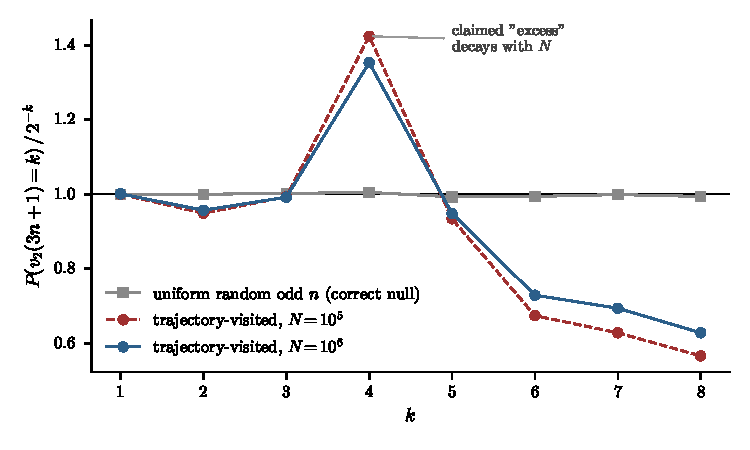
\includegraphics[width=\textwidth]{fig_v2_ratios.pdf}
\caption{Ratio of the observed $v_2(3n+1)$ distribution to $2^{-k}$. Over uniform random odd $n$ (squares) the ratio is $1$ throughout. Over trajectory-visited odds the apparent excess at $k=4$ and deficit at large $k$ both decay toward $1$ as $N$ grows.}
\label{fig:v2}
\end{figure}

\subsection{Case 3. The prime/composite gap is a parity confound}\label{sec:primes}

The raw comparison shows primes averaging $4.1\%$ longer trajectories than composites ($136.41$ versus $131.01$ steps), and is sometimes reported as a primality effect. It is a parity artifact. Every prime except $2$ is odd, composites are mostly even, and odd starting values have systematically longer trajectories because an odd start must climb through $3n+1$ before it can descend. Controlling for parity reverses the sign: odd primes average $136.41$ steps against $137.82$ for odd composites, a gap of $-1.0\%$ (difference $-1.41$ steps, $95\%$ CI $[-1.84, -0.97]$). The residual is a size effect: within decade bands (Figure~\ref{fig:parity}) the odd-prime versus odd-composite gap shrinks monotonically from $-3.7\%$ on $[10^2, 10^3)$ to $-0.3\%$ on $[10^5, 10^6)$. We find no primality effect beyond the parity and size composition of the two groups.

\begin{figure}[ht]
\centering
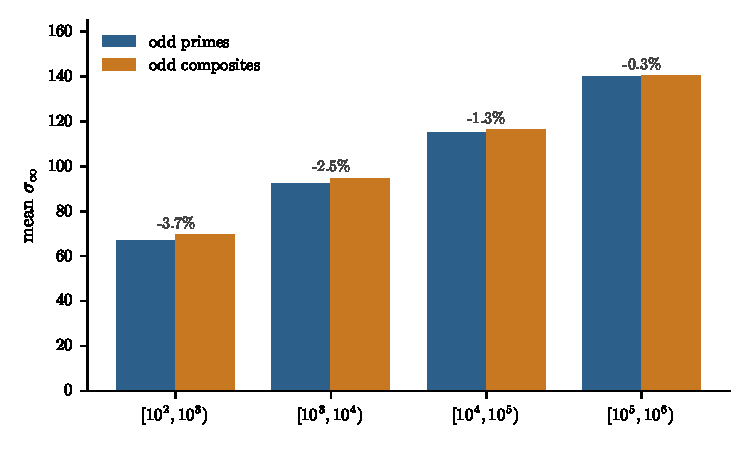
\includegraphics[width=\textwidth]{fig_prime_parity.pdf}
\caption{Mean total stopping time by decade for odd primes and odd composites. Once parity is controlled, the gap nearly vanishes and shrinks further with size.}
\label{fig:parity}
\end{figure}

\subsection{Case 4. The Sophie Germain ratio is a dominated estimator}\label{sec:sg}

An earlier version of this analysis reported that for Sophie Germain primes $p$ (primes with $2p+1$ also prime), the ratio $\sigma_\infty(2p+1)/\sigma_\infty(p)$ averages near $1.328 \approx 4/3$, read as a link between prime structure and trajectory dynamics. Three controls dissolve it (Table~\ref{tab:sg}). First, the statistic is a mean of ratios over $p \le 50{,}000$, and a mean of ratios is dominated by small denominators: $p = 2$ contributes $\sigma_\infty(5)/\sigma_\infty(2) = 5.0$ and $p = 23$ contributes $104/15 \approx 6.9$. The median ratio is $1.01$ and the ratio of means is $1.11$. Second, the same statistic on non-Sophie-Germain primes gives $1.338$, and on odd composites $1.310$, indistinguishable from the Sophie Germain value: the number measures the map $m \mapsto 2m+1$ under a skew-sensitive estimator, not Sophie Germain structure. Third, the value is unstable in the cap: extending to $p \le 5 \times 10^5$ moves the mean of ratios to $1.23$ for all three groups alike. We note in passing that the original reading also equated $4/3 = 1.333$ with $\log 4 / \log 3 \approx 1.262$, two different numbers five percent apart.

\begin{table}[ht]
\centering
\caption{The ``Sophie Germain ratio'' under the map $m \mapsto 2m+1$, same statistic for three groups, $m \le 50{,}000$. The value is reproduced by groups with no Sophie Germain structure.}
\label{tab:sg}
\small
\begin{tabular}{lrccc}
\toprule
Group & $n$ & Mean of ratios & Median & Ratio of means \\
\midrule
Sophie Germain primes & $670$ & $1.328$ & $1.012$ & $1.107$ \\
Non-SG primes & $4{,}463$ & $1.338$ & $1.012$ & $1.138$ \\
Odd composites & $19{,}867$ & $1.310$ & $1.011$ & $1.121$ \\
\bottomrule
\end{tabular}
\end{table}

Two related observations fall to the same controls. The mean absolute difference in total stopping time between twin primes $(p, p+2)$ is $47.97$ steps, but a matched control of consecutive odd numbers shows the same spread (twin-to-control ratio $1.008$), so the dispersion is the ordinary step-to-step variance of the map, not a property of twins. And the ordering of mean stopping time by residue class modulo $6$ (lowest for multiples of $6$ near $119$, highest for $n \equiv 5$ near $142$) is fully accounted for by the parity mix and $3$-divisibility of each class, not an anomaly to be explained further.

\section{The hardest case: our own funnel conjecture}\label{sec:capstone}

The protocol is easy to state and harder to apply to a conclusion one would like to keep. We close the analysis by applying it to the one claim we still believed after the four above.

The residual deviation from Benford in Table~\ref{tab:digits} is small but it is not nothing, and it is not generic. A matched multiplicative random walk ($\times 3/2$ or $\times 1/2$ with equal probability) reaches $\TVD < 0.001$ from Benford over a comparable number of values, so the deviation is not a generic property of finite multiplicative processes. We conjectured a specific cause: the low-altitude values that every trajectory must traverse near the terminal cycle ($\dots, 16, 8, 4, 2, 1$ and their neighbours) appear in every pooled trajectory, carry a fixed non-Benford digit profile, and so should drag the pooled histogram off Benford by an amount that shrinks like $1/\log N$ as trajectories lengthen.

The conjecture makes one falsifiable prediction. If the shared low-altitude values are the cause, then removing them should move the remaining distribution \emph{toward} Benford. Table~\ref{tab:excision} reports the test. Removing them moves the distribution \emph{away} from Benford: the full multi-decade pool is the configuration closest to Benford, and truncating it from below raises the total variation distance, from $0.0198$ to $0.0456$ by the time values under $10^3$ are excluded. The prediction is false. The shared low-altitude values are not the source of the deviation; the funnel dominates the population of pooled values, with $39\%$ of them below $10^3$, but it does not dominate the deviation. We had conflated those two facts. We ran the test that we expected to confirm our explanation, and it eliminated it.

\begin{table}[ht]
\centering
\caption{Excision test at $N = 10^6$. Removing the small values raises the deviation from Benford rather than lowering it, refuting the shared-funnel explanation.}
\label{tab:excision}
\begin{tabular}{lrr}
\toprule
Values retained & Share of pool & $\TVD$ from Benford \\
\midrule
all & $100\%$ & $0.0198$ \\
$\ge 10^2$ & $84\%$ & $0.0221$ \\
$\ge 10^3$ & $61\%$ & $0.0456$ \\
$\ge 10^4$ & $39\%$ & $0.0502$ \\
$\ge 10^5$ & $22\%$ & $0.0940$ \\
\bottomrule
\end{tabular}
\end{table}

What remains after the mechanism is withdrawn is a smaller and more careful statement. The part of the deviation specific to the map is a per-digit signature, an excess at leading digit $4$ and a deficit at digit $6$, that a structureless reference does not produce. We measured it against a scale-invariant null drawn over the same span of magnitudes; that null carries a comparable total variation distance but its per-digit deviations stay within a few percent and never single out digit $4$, and it is itself non-monotonic in $N$ because it depends on the fractional number of decades spanned. For that reason we read the signature directly rather than through a difference against the null. Table~\ref{tab:signature} tracks it across the same four decades as Table~\ref{tab:tvd}. The signature decreases monotonically: the digit-$4$ excess falls from $32.7\%$ to $15.0\%$ and the digit-$6$ deficit from $26.5\%$ to $12.3\%$ across a thousandfold increase in range. It decreases, moreover, where the boundary-phase null does not, which is the evidence that its decrease is convergence and not phase.

\begin{table}[ht]
\centering
\caption{The map-specific per-digit signature across range. It decreases monotonically over four decades, unlike the scale-invariant null, whose total variation distance is non-monotonic.}
\label{tab:signature}
\begin{tabular}{rrrr}
\toprule
$N$ & Digit-4 excess & Digit-6 deficit & Null $\TVD$ \\
\midrule
$10^3$ & $+32.7\%$ & $-26.5\%$ & $0.0385$ \\
$10^4$ & $+23.9\%$ & $-18.6\%$ & $0.0303$ \\
$10^5$ & $+18.2\%$ & $-14.8\%$ & $0.0148$ \\
$10^6$ & $+15.0\%$ & $-12.3\%$ & $0.0155$ \\
\bottomrule
\end{tabular}
\end{table}

By the standard of this paper, a feature that decreases monotonically over four decades, in step with the proven asymptotic convergence of Kontorovich and Miller \cite{km2005}, is finite-range. We state it as that and no more. We do not claim that nothing whatever survives in the limit, only that the last candidate, like the four before it, decreases rather than persists as the range grows. We include the episode as the central illustration of the protocol, because the two temptations it required us to resist, dressing a finite-range feature in a mechanism the data did not support, and then rounding a decreasing residual down to a clean zero so that the sweep would look complete, are exactly the failure modes this paper is about, and they are the ones we came closest to committing.

\section{Discussion}\label{sec:discussion}

The four candidate anomalies and our own fifth conjecture fail in three distinct ways, one for each rule. The $2$-adic excess fails the null: it measures the visited sample, not the map. The Benford violation fails the effect-size rule: its $\chi^2$ is a statement about the pooled count. The prime/composite gap and the Sophie Germain ratio fail under the obvious confounders of parity, size, and estimator skew. And the funnel conjecture fails its own direct test. In every case the corrected statement is consistent with the standard heuristic model and the proven asymptotic theorems: odd steps multiply by about $3/2$, even steps halve, $v_2$ over odd $n$ is geometric, and leading digits approach Benford at finite range from a measurable, decreasing distance.

The general lesson is procedural and applies beyond this map. At pooled sample sizes of order $10^8$, significance tests are uninformative and the choice of null model decides the conclusion, so the null must be fixed before measuring and the effect reported as a size rather than a $p$-value. Estimators that a few terms can dominate should be checked against their median and their pooled analogue. And any candidate anomaly should be required to survive a tenfold, preferably thousandfold, increase in range before it is named, with ``survives'' meaning that the effect, measured the same way at every scale, does not decay. The discipline costs little to apply and, as our own fifth case shows, it is most needed precisely when one has grown attached to the answer.

\section{Conclusion}

We set out a three-rule protocol for distinguishing genuine structure in Collatz trajectory statistics from artifacts of method, and applied it without exception to five candidate anomalies, four from the surrounding literature and one of our own. None survives. The leading-digit deviation from Benford is small and decreasing; the $2$-adic excess is a wrong-null artifact; the prime/composite gap is parity; the Sophie Germain ratio is a dominated estimator; and the shared-funnel mechanism we proposed for the last residual is refuted by its own excision test, leaving a real but monotonically decreasing per-digit signature that we decline to over-read. The result is not a discovery about the Collatz map. It is a demonstration that, at the scales typical of computational work on this problem, the protocol and not the data decides what counts as an anomaly, and that the protocol must be applied to one's own conclusions most of all.

\section*{Code availability}\label{sec:code}

All analysis code is written in Python and is available at \url{https://github.com/SoDonik/collatz-anomaly-protocol}, archived as version v1.0.0 at Zenodo, \url{https://doi.org/10.5281/zenodo.20723339}. Every audited number in Sections \ref{sec:cases} and \ref{sec:capstone} is reproducible from a single verification script that recomputes the tables from scratch, including the four-point scale series and the excision test; the complete suite runs in minutes on consumer hardware using a memoized trajectory recurrence.

\begin{thebibliography}{9}

\bibitem{lagarias1985}
J.~C. Lagarias, \emph{The $3x+1$ problem and its generalizations}, Amer. Math. Monthly \textbf{92} (1985), no.~1, 3--23.

\bibitem{lagariasweiss1992}
J.~C. Lagarias and A.~Weiss, \emph{The $3x+1$ problem: two stochastic models}, Ann. Appl. Probab. \textbf{2} (1992), no.~1, 229--261.

\bibitem{applegate1995}
D.~Applegate and J.~C. Lagarias, \emph{Density bounds for the $3x+1$ problem}, Math. Comp. \textbf{64} (1995), no.~209, 411--426.

\bibitem{km2005}
A.~V. Kontorovich and S.~J. Miller, \emph{Benford's law, values of $L$-functions and the $3x+1$ problem}, Acta Arith. \textbf{120} (2005), no.~3, 269--297.

\bibitem{ls2006}
J.~C. Lagarias and K.~Soundararajan, \emph{Benford's law for the $3x+1$ function}, J. London Math. Soc. \textbf{74} (2006), no.~2, 289--303.

\bibitem{kl2009}
A.~V. Kontorovich and J.~C. Lagarias, \emph{Stochastic models for the $3x+1$ and $5x+1$ problems}, in \emph{The Ultimate Challenge: The $3x+1$ Problem}, Amer. Math. Soc., Providence, RI, 2010, pp.~131--188.

\bibitem{tao2019}
T.~Tao, \emph{Almost all orbits of the Collatz map attain almost bounded values}, Forum Math. Pi \textbf{10} (2022), e12; arXiv:1909.03562.

\bibitem{barina2021}
D.~Barina, \emph{Convergence verification of the Collatz problem}, J. Supercomput. \textbf{77} (2021), 2681--2688.

\bibitem{cerqueti2023}
R.~Cerqueti and C.~Lupi, \emph{Severe testing of Benford's law}, TEST \textbf{32} (2023), no.~2, 677--694. \texttt{DOI:10.1007/s11749-023-00848-z}.

\bibitem{kossovsky2021}
A.~E. Kossovsky, \emph{On the mistaken use of the chi-square test in Benford's law}, Stats \textbf{4} (2021), no.~2, 419--453. \texttt{DOI:10.3390/stats4020027}.

\end{thebibliography}

\end{document}
